\chapter{Methods}

\section{Robotic Platform}

The focus of this work is the application of tracking in humanoid robotic platforms, where the manipulator is observed in a camera frame which is part of the robot's kinematic chain.

\subsection{Hardware}

The applied robot platform the the humanoid robot Valkyrie which is developed by NASA (\cref{fig:valkyrie}). It is \SI{1.8}{\meter} high and weights about \SI{125}{\kilo\gram}. In totally, it is actuated by 58 joints: leg ($2 \times 6$), arms ($2 \times 7$), hands ($2 \times 13$), neck (3) and torso (3). Hence, the kinematic chain from the observation frame to the hand frame consists of 10 actuated joints.

\begin{figure}
%\centering
\begin{minipage}{0.5\textwidth}
\centering
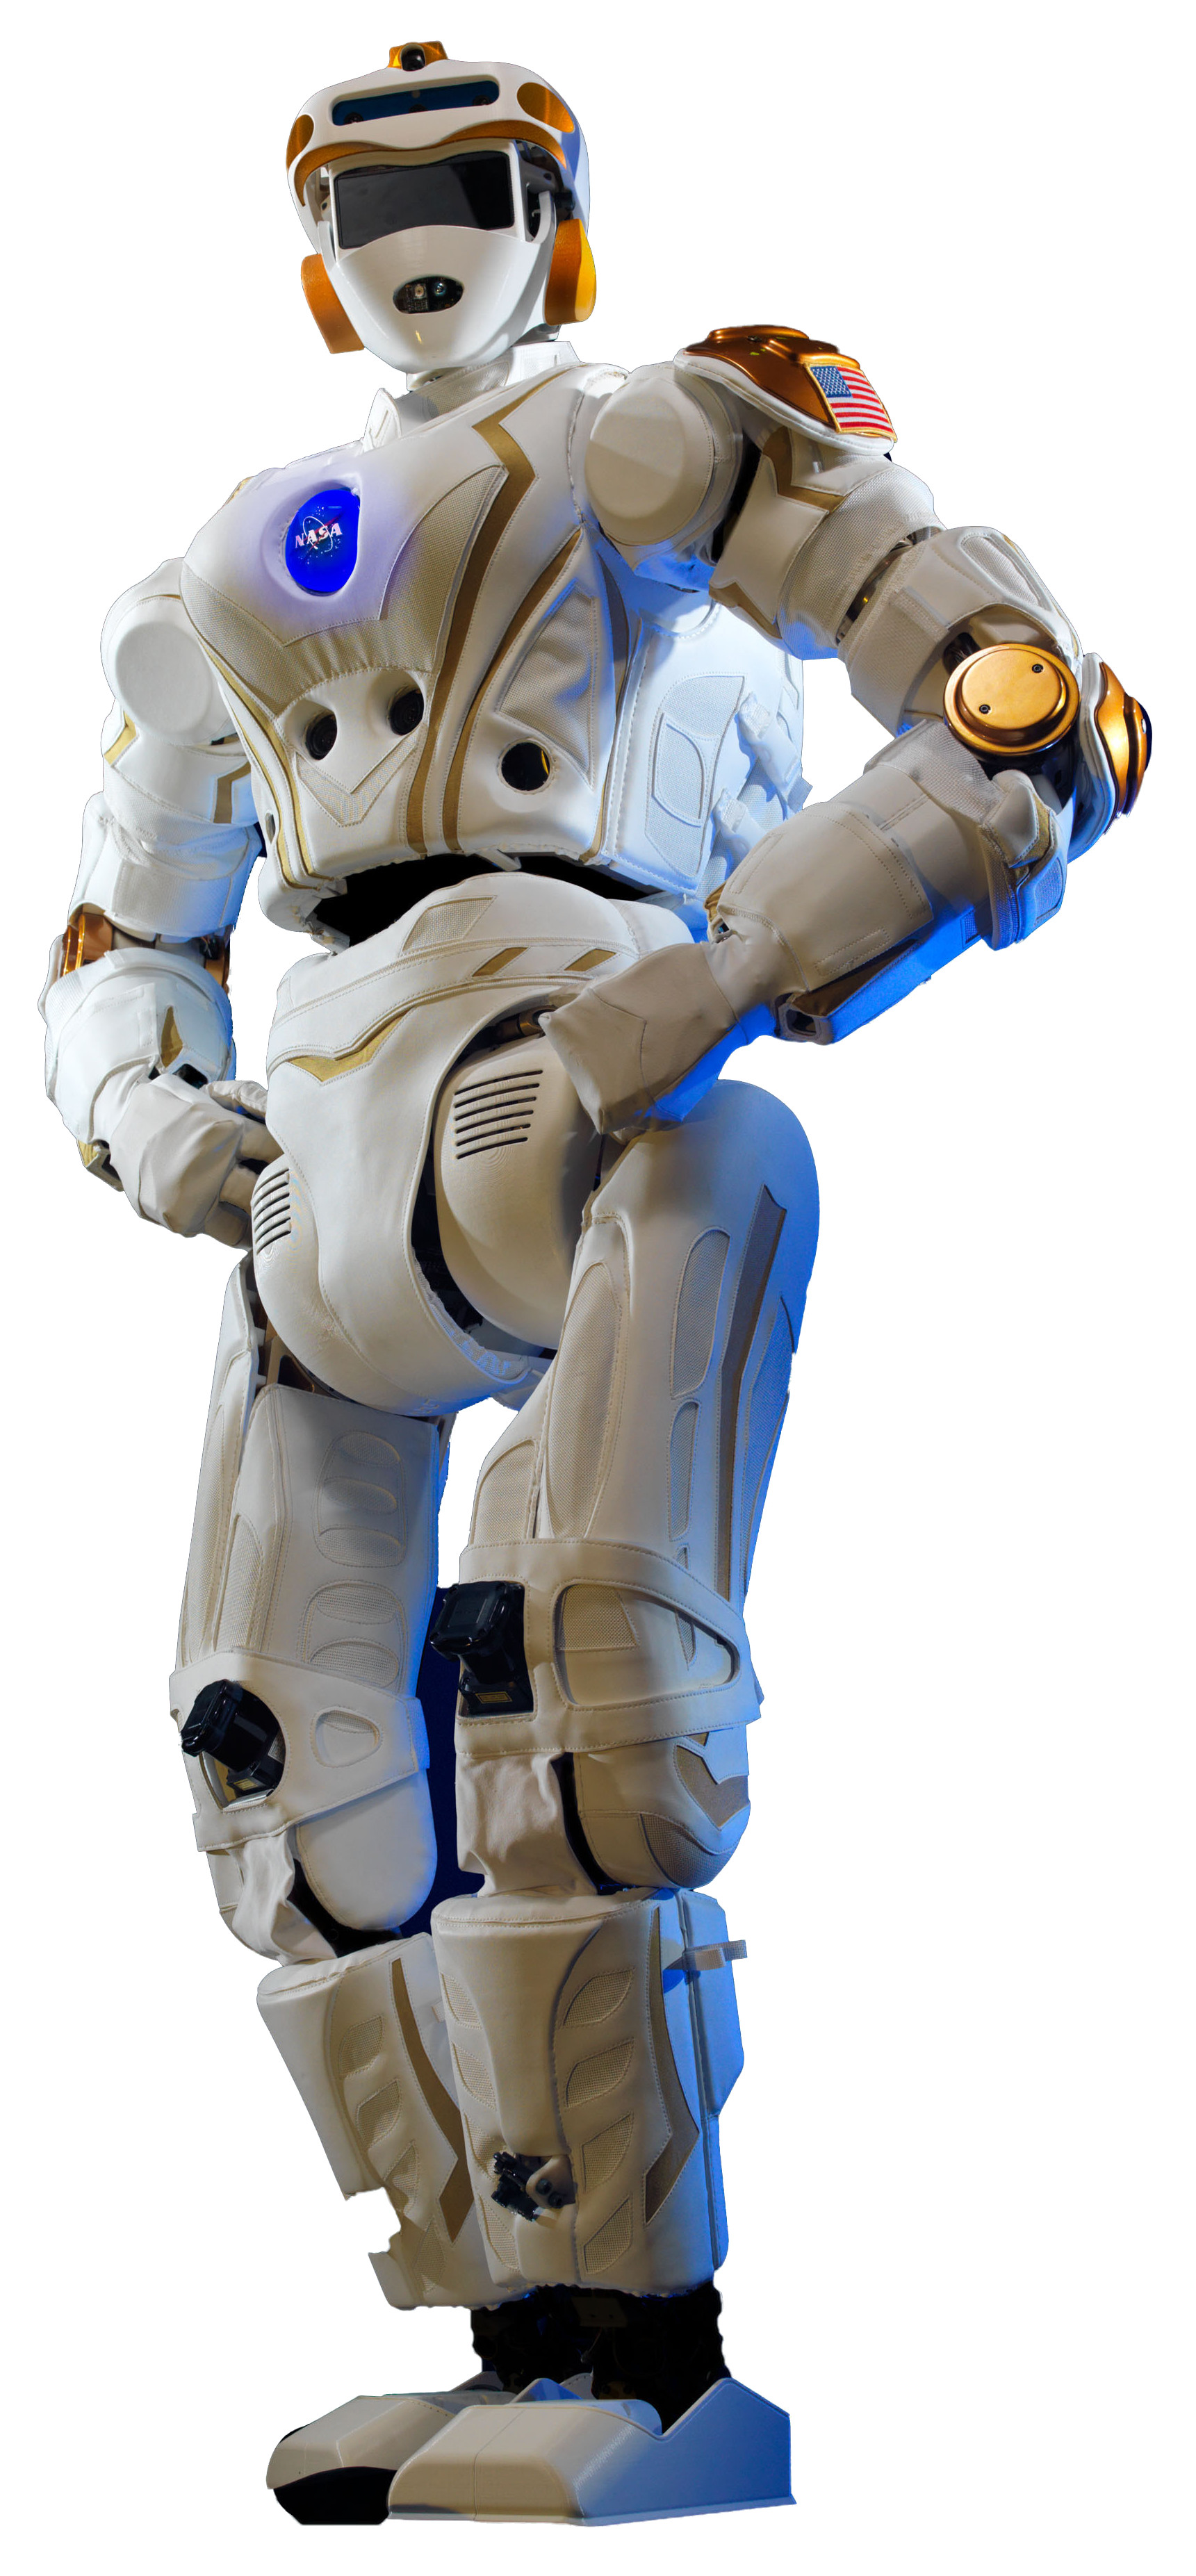
\includegraphics[width=0.6\textwidth]{images/valkyrie/Valkyrie.jpg}
\caption{Humanoid robot Valkyrie (Image credits: NASA)}
\label{fig:valkyrie}
\end{minipage}
%
\hspace{0.5cm}
%
\begin{minipage}{0.5\textwidth}
\centering
\subfloat[MultiSense SL]{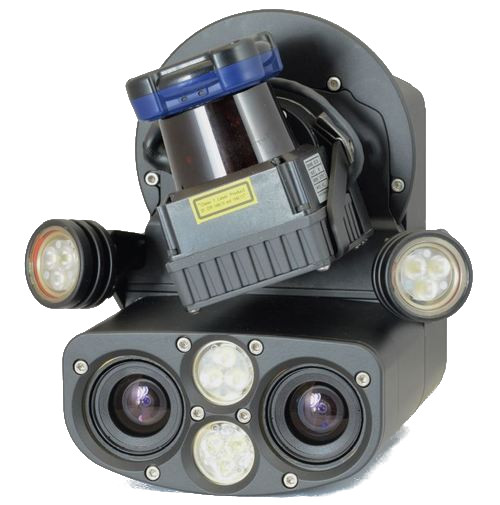
\includegraphics[width=0.8\textwidth]{images/valkyrie/MultiSense_SL.jpg} \label{fig:multisense}}

\subfloat[Asus Xtion PRO]{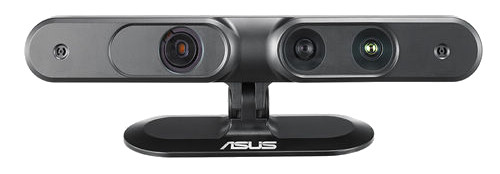
\includegraphics[width=0.8\textwidth]{images/valkyrie/xtion_pro_live.jpg} \label{fig:xtion_pro}}
\caption{Depth perception systems (Image credits: (a) Carnegie Robotics, (b) Asus)}
\label{fig:depth_sensors}
\end{minipage}
\end{figure}

The robot will use depth data as its main source of information for estimating the configuration of the manipulator and the object pose. The MultiSense SL stereo and LIDAR depth sensor (\cref{fig:multisense}), which is mounted inside the head of the robot, provides two source of depth image from (1) stereo matching at \SI{15}{\hertz}, and (2) a rotating LIDAR which generates a fill scan at \nicefrac{1}{6} \si{\hertz}. An optional structure from light sensor (\cref{fig:xtion_pro}), which can be mounted on top of the head, uses the known location of projected IR dots to estimate the depth at these locations. The stereo cameras have its IR filter removed to enhance stereo matching by providing distinct keypoints from the IR pattern. The LIDAR data is not applied for tracking because of its low update rate.
The key properties of both depth sensors are compared in \cref{tab:depth_sensor_comparison}. These properties are used to back-project the disparity values into the 3D points.

\begin{table}
\captionsetup{width=0.7\textwidth}
\centering
\begin{tabular}{|c||c|c|}
\hline
 & \textit{MultiSense SL} & \textit{Asus Xtion PRO Live} \\
\hline
\hline
depth range & \SI{0.4}{\meter} - \SI{10}{\meter} & \SI{0.8}{\meter} - \SI{3.5}{\meter} \\
\hline
FOV & \SI{80}{\degree} $\times$ \SI{45}{\degree} & \SI{58}{\degree} $\times$ \SI{45}{\degree} \\
\hline
resolution & $1024 \times 1024$ & $640 \times 480$ \\
\hline
FPS & \SI{15}{\hertz} & \SI{30}{\hertz} \\
\hline
%f & \SI{6.5}{\milli\meter} & • \\
%\hline
$f_x$, $f_y$ & \SI{556.183}{pxl} & \SI{528.014}{pxl} \\
\hline
$c_x$, $c_y$ & \SI{512}{pxl} & (\SI{320}{pxl}, \SI{267}{pxl}) \\
\hline
b & \SI{0.07}{\meter} & \SI{0.075}{\meter} \\
\hline
\end{tabular}
\caption[Comparison of depth sensors]{Comparison of depth sensors. FOV: field of view, FPS: frames per second, $f$: focal length, $c$: image centre, $b$: baseline}
\label{tab:depth_sensor_comparison}
\end{table}


\subsection{Robot Model Representation}

Part of this thesis is the adaptation of the reference implementation to robot model representations stored in the URDF (Unified Robot Description Format) format. URDF defines at a minimum a tree structure that resembles the kinematic tree of a robot with its joints and links. In addition it can provide, among other things, information about joint limits and the geometric properties of the links. These geometric properties can be defined as primitive shapes like spheres, boxes or cylinders, or alternatively refer to complexer triangle meshes.

The URDF plugin for DART is designed that way, that all parts of the kinematic chain that are connected to a given root frame are tracked. This enables us to neglect robot parts that are not involved in manipulation. \cref{fig:val_model_dart} shows such a model that is loaded from the \texttt{torso} frame upwards in the kinematic tree. Hence, it includes both arms, hands and the head with the sensors. This enables us to track both hands in a bi-manual grasping task with respect to the camera frame without invalidating kinematic constraints, such as overrunning joint limits or disconnecting links.

\begin{figure}
\centering
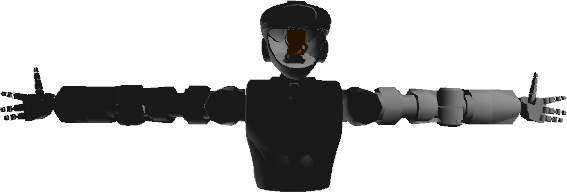
\includegraphics[width=\textwidth]{images/valkyrie/val_model_torso_dart.png}
\caption{Robot model loaded in DART}
\label{fig:val_model_dart}
\end{figure}


\section{Signed Distance Function}

The descriptions in this section of the thesis are based on work by Schmidt et al. \cite{Schmidt2015} that presents the DART algorithm.

The signed distance function (SDF) gives the shortest distance of a point in the observed point cloud to the robot model. It is signed in the sense that the distance is positive if the point lies outside the model, it is negative if the point is inside the model, and it is zero if the point lies exactly on the surface of the model. DART uses two kind of SDFs: the model SDF and the observation SDF.

The model SDF (\cref{fig:model_SDF}) gives the shortest distance of a point to a rigid model mesh. For articulated models, which consist of multiple such model meshes, a local model SDF is applied. This way, the complex computation of a global model SDF for each articulation can be broken down to the parallel computation of local SDF per robot part. For each point in the point cloud data, the distance to each robot part, respectively frame, is computed using the precomputed local SDFs. The point is then associated to the robot frame with the smallest absolute distance value.

In addition to considering observed data and the robot model, which is defined as \textit{positive information} in DART, the optimization is also using \textit{negative information}. If a point is observed in 3D, there cannot be anything in between this point and the camera centre. This free space constrain is visualised in \cref{fig:observation_SDF}. This observation SDF uses the distance transform on the observation and the estimated configuration of the model from the model SDF to constrain models to not be in free space.

\begin{figure}
\centering
\subfloat[Model SDF]{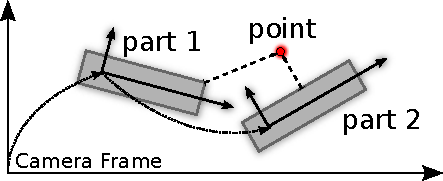
\includegraphics[width=0.5\textwidth]{images/sdf/local_sdf.pdf} \label{fig:model_SDF}}
\subfloat[Observation SDF]{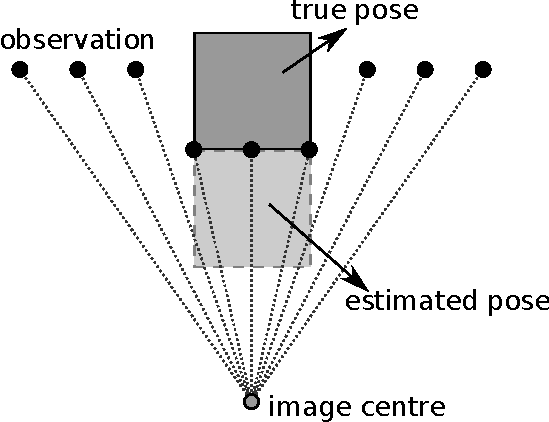
\includegraphics[width=0.3\textwidth]{images/sdf/sdf_obs.pdf} \label{fig:observation_SDF}}
\caption[Signed Distance Function]{Local model SDF and observation SDF (Inspired by \cite{Schmidt2015} figures 3 and 6). (a) the observed point is assigned to \emph{part 2}, (b) the estimated box (light gray) lies in between the observation and the image centre and thus invalidates the free space constrain.}
\end{figure}

\section{Gauss-Newton Algorithm}

The \textit{Gauss-Newton} algorithm is a method for finding the optimal set of parameters $\mathbf{p}$ that minimizes the sum of squares of non-linear vector-valued objective functions $e(\cdot)$
%
\begin{equation}
\hat{\mathbf{p}} = \arg\min_{p} \sum_{i=1}^N\left[ e_i(\mathbf{p})^2\right] .
\end{equation}

The Gauss-Newton algorithm is derived from the \textit{Newton} algorithm for finding roots and extremal points which itself is based on the Taylor series expansion. The Newton method for finding extremal points of the scalar objective function $f(x)$ is an iterative procedure
%
\begin{equation}
x_{t+1} = x_t - \frac{f^{(1)}(x_t)}{f^{(2)}(x_t)}
\label{eqn:newton_minimum}
\end{equation}
%
starting at an initial state $x_0$ using the first- and second-order derivatives ($f^{(1)}$, $f^{(2)}$) of the objective function.

For finding the minimum of the function $e(\cdot)$ with respect to a parameter vector $\mathbf{p}$, the first- and second-order partial derivatives are used. In particular, the first- and second-order derivatives in \ref{eqn:newton_minimum} are replaced by the gradient $\nabla e(\mathbf{p})$ and the Hessian $\nabla^2 e(\mathbf{p})$ of the objective function $e$.
The partial derivatives of the vector-valued function $e(\cdot)$ with respect to the parameter vector $\mathbf{p}$ are aggregated in the \textit{Jacobian} matrix $J\in \mathbb{R}^{i \times j}$ with elements
%
\begin{equation}
J_{i,j} = \frac{\partial e_i(\mathbf{p})}{\partial p_j} .
\end{equation}
%
Hence,
\begin{align}
\nabla e(\mathbf{p}) &= J^\top e(\mathbf{p}) \label{eqn:gn_gradient}\\
H(e) = \nabla^2 e(\mathbf{p}) &= J^\top J +  \sum_{i=1} e_i(\mathbf{p}) \nabla^2 e_i(\mathbf{p}) \label{eqn:gn_hessian_full}.
\end{align}

For small $e$, the Hessian $H(e)$ can be approximated by
\begin{equation}
H(e) \approx J^\top J \label{eqn:gn_hessian}
\end{equation}
%
neglecting the second-order derivatives. This approximation is used in the Gauss-Newton algorithm and the parameter update step becomes
%
\begin{align}
\mathbf{p}_{t+1} &= \mathbf{p}_{t} - \Delta\mathbf{p} \\
&= \mathbf{p}_{t} - H(e)^{-1} \cdot \nabla e(\mathbf{p}) \\
&= \mathbf{p}_{t} - \left(J^\top J\right)^{-1} \cdot J^\top e(\mathbf{p}) \label{eqn:gn_param_update}.
\end{align}

The parameter update $\Delta\mathbf{p}$ is proportionally driven by the gradient of the objective function and inverse proportional by the approximation of the Hessian.


\section{Prior Information}

Prior information can be used in the Gauss-Newton algorithm by modulating the Hessian approximation and the gradient towards the desired state. This is achieved by selecting an objective function and calculating its partial derivatives with respect to the parameter vector. These partial derivatives are used in the Jacobian as shown in equations \ref{eqn:gn_gradient} and \ref{eqn:gn_hessian}.

The full parameter vector in DART consists of the 6D pose of the root frame and the $N$ joints positions:
\begin{equation}
\mathbf{p} = \begin{bmatrix}
x & y & z & \phi & \theta & \psi & | & q_1 & \cdots & q_N
\end{bmatrix}
\end{equation}

with $x$, $y$, $z$ for the translation, $\phi$, $\theta$, $\psi$ for the orientation in radiant Euler angles, and $q_1 \dots q_N$ the individual joint position values.


\subsection{Known Frame Pose}

For constraining the translation of the root frame in between optimization iterations, the parameter update vector $\Delta\mathbf{p}$ must be computed such that its first 6 elements for the pose are $0$. From equation \ref{eqn:gn_param_update}
\begin{align}
\Delta\mathbf{p} &= \left(J^\top J\right)^{-1} \cdot J^\top e(\mathbf{p}) = \begin{bmatrix}
\mathbf{0} & | & q_1 & \cdots & q_N
\end{bmatrix} \\
J^\top e &= J^\top J \cdot \begin{bmatrix}
\mathbf{0} & | & q_1 & \cdots & q_N
\end{bmatrix}
\end{align}

Cancelling out the pose update can be achieved by applying the prior on the final blended Hessian and gradient just before the final parameter update is computed. In particular the fixed frame prior computes the parameter update $\Delta\mathbf{p}$ from the blended Hessian and gradient, cancels out the first 6 elements for the pose, and computes the new gradient. Instead of blending this gradient ($J^\top e$) into the final gradient, the global gradient is overwritten resulting in enforcing no frame pose update.


\subsection{Reported Joint Positions}

We use the reported state of the robot in a way, that we can drag the estimated solution away from possibly distracting perceptions towards the state perceived through the joint encoders.
%
Three different kind of objective functions have been selected for this purpose which compute a weighted deviation of the estimated joint configuration $\mathbf{q}$ from reported joint configuration $\mathbf{r}$. For all objective functions, $r_i$ and $q_i$ denote the individual joint positions in their corresponding configuration vector.

\begin{enumerate}
\item Weighted L2 norm of the estimated joint position deviation:
\begin{equation}
e_1 = w \cdot \lVert \mathbf{r} - \mathbf{q} \rVert = w \cdot \sqrt{\sum_{i=1}^N (r_i - q_i)^2} \label{eqn:objf_weightedL2}
\end{equation}
with scalar weight $w>0$.

\item L2 norm of the weighted joint deviation:
\begin{equation}
e_2 = \lVert w \cdot (\mathbf{r} - \mathbf{q}) \rVert = \sqrt{\sum_{i=1}^N w \cdot (r_i - q_i)^2} \label{eqn:objf_L2ofweighted}
\end{equation}
with the same scalar weight $w>0$ for all joint deviations.

\item Sum of squares of individually weighted joints:
\begin{equation}
e_3 = \lvert \mathbf{r} - \mathbf{q} \rvert^\top Q \lvert \mathbf{r} - \mathbf{q} \rvert = \sum_{i=1}^N \left[ (r_i-q_i) \cdot \sum_{j=1}^N (r_j-q_j) \cdot \omega_{i,j} \right] \label{eqn:objf_indiv_weighted}
\end{equation}
with the weight matrix $Q\in\mathbf{R}^{N\times N}$ and its elements $\omega_{i,j}$. As a error metric, the weight matrix $Q$ must be \emph{positive-semidefinite}. That is, $\forall \mathbf{x}\in\mathbf{R}^n: x^\top Q x \geq 0$.
\end{enumerate}

Whereas the first two objective functions (\ref{eqn:objf_weightedL2} and \ref{eqn:objf_L2ofweighted}) use a common scalar weight for all joint deviations, the third objective function (\ref{eqn:objf_indiv_weighted}) can apply different weights per joint and hence enables to penalize whole parts of the kinematic chain more precise.

The respective partial derivatives for the Jacobian are:
\begin{enumerate}
\item Weighted L2 norm of the estimated joint position deviation
\begin{equation}
J_{ji} = \frac{\partial e_1}{\partial q_i} = -w \frac{r_i - q_i}{\lVert \mathbf{r} - \mathbf{q} \rVert}
\end{equation}

\item L2 norm of the weighted joint deviation:
\begin{equation}
J_{ji} = \frac{\partial e_2}{\partial q_i} = -w^2 \frac{r_i - q_i}{\lVert w \cdot (\mathbf{r} - \mathbf{q}) \rVert}
\end{equation}

\item Sum of squares of individually weighted joints:
\begin{equation}
J_{ji} = \frac{\partial e_3}{\partial q_i} = - \left[ \sum_{j=1}^N d_jq_{i,j}\right] + \left[ \sum_{j=1 \neq i}^N d_jq_{j,i}\right]
\end{equation}
\end{enumerate}


\section{Ground Truth Data Collection}

To evaluate the tracking performance and verify the effect of the joint position prior, reference measurements of the true state of the robot are required. The Vicon motion caption system is selected to externally track the pose of IR reflective markers rigidly attached to the robot.

\subsection{Setup}

To obtain the true transformation from the pelvis frame to the left hand palm frame, reflective markers are rigidly mounted with standoffs to the specific robot frames. The photograph in \cref{fig:vicon_marker} shows the highlighted location of the markers on the \texttt{pelvis} frame (green) and the \texttt{leftPalm} frame (red).

\begin{figure}
\captionsetup{width=0.4\textwidth}
\centering
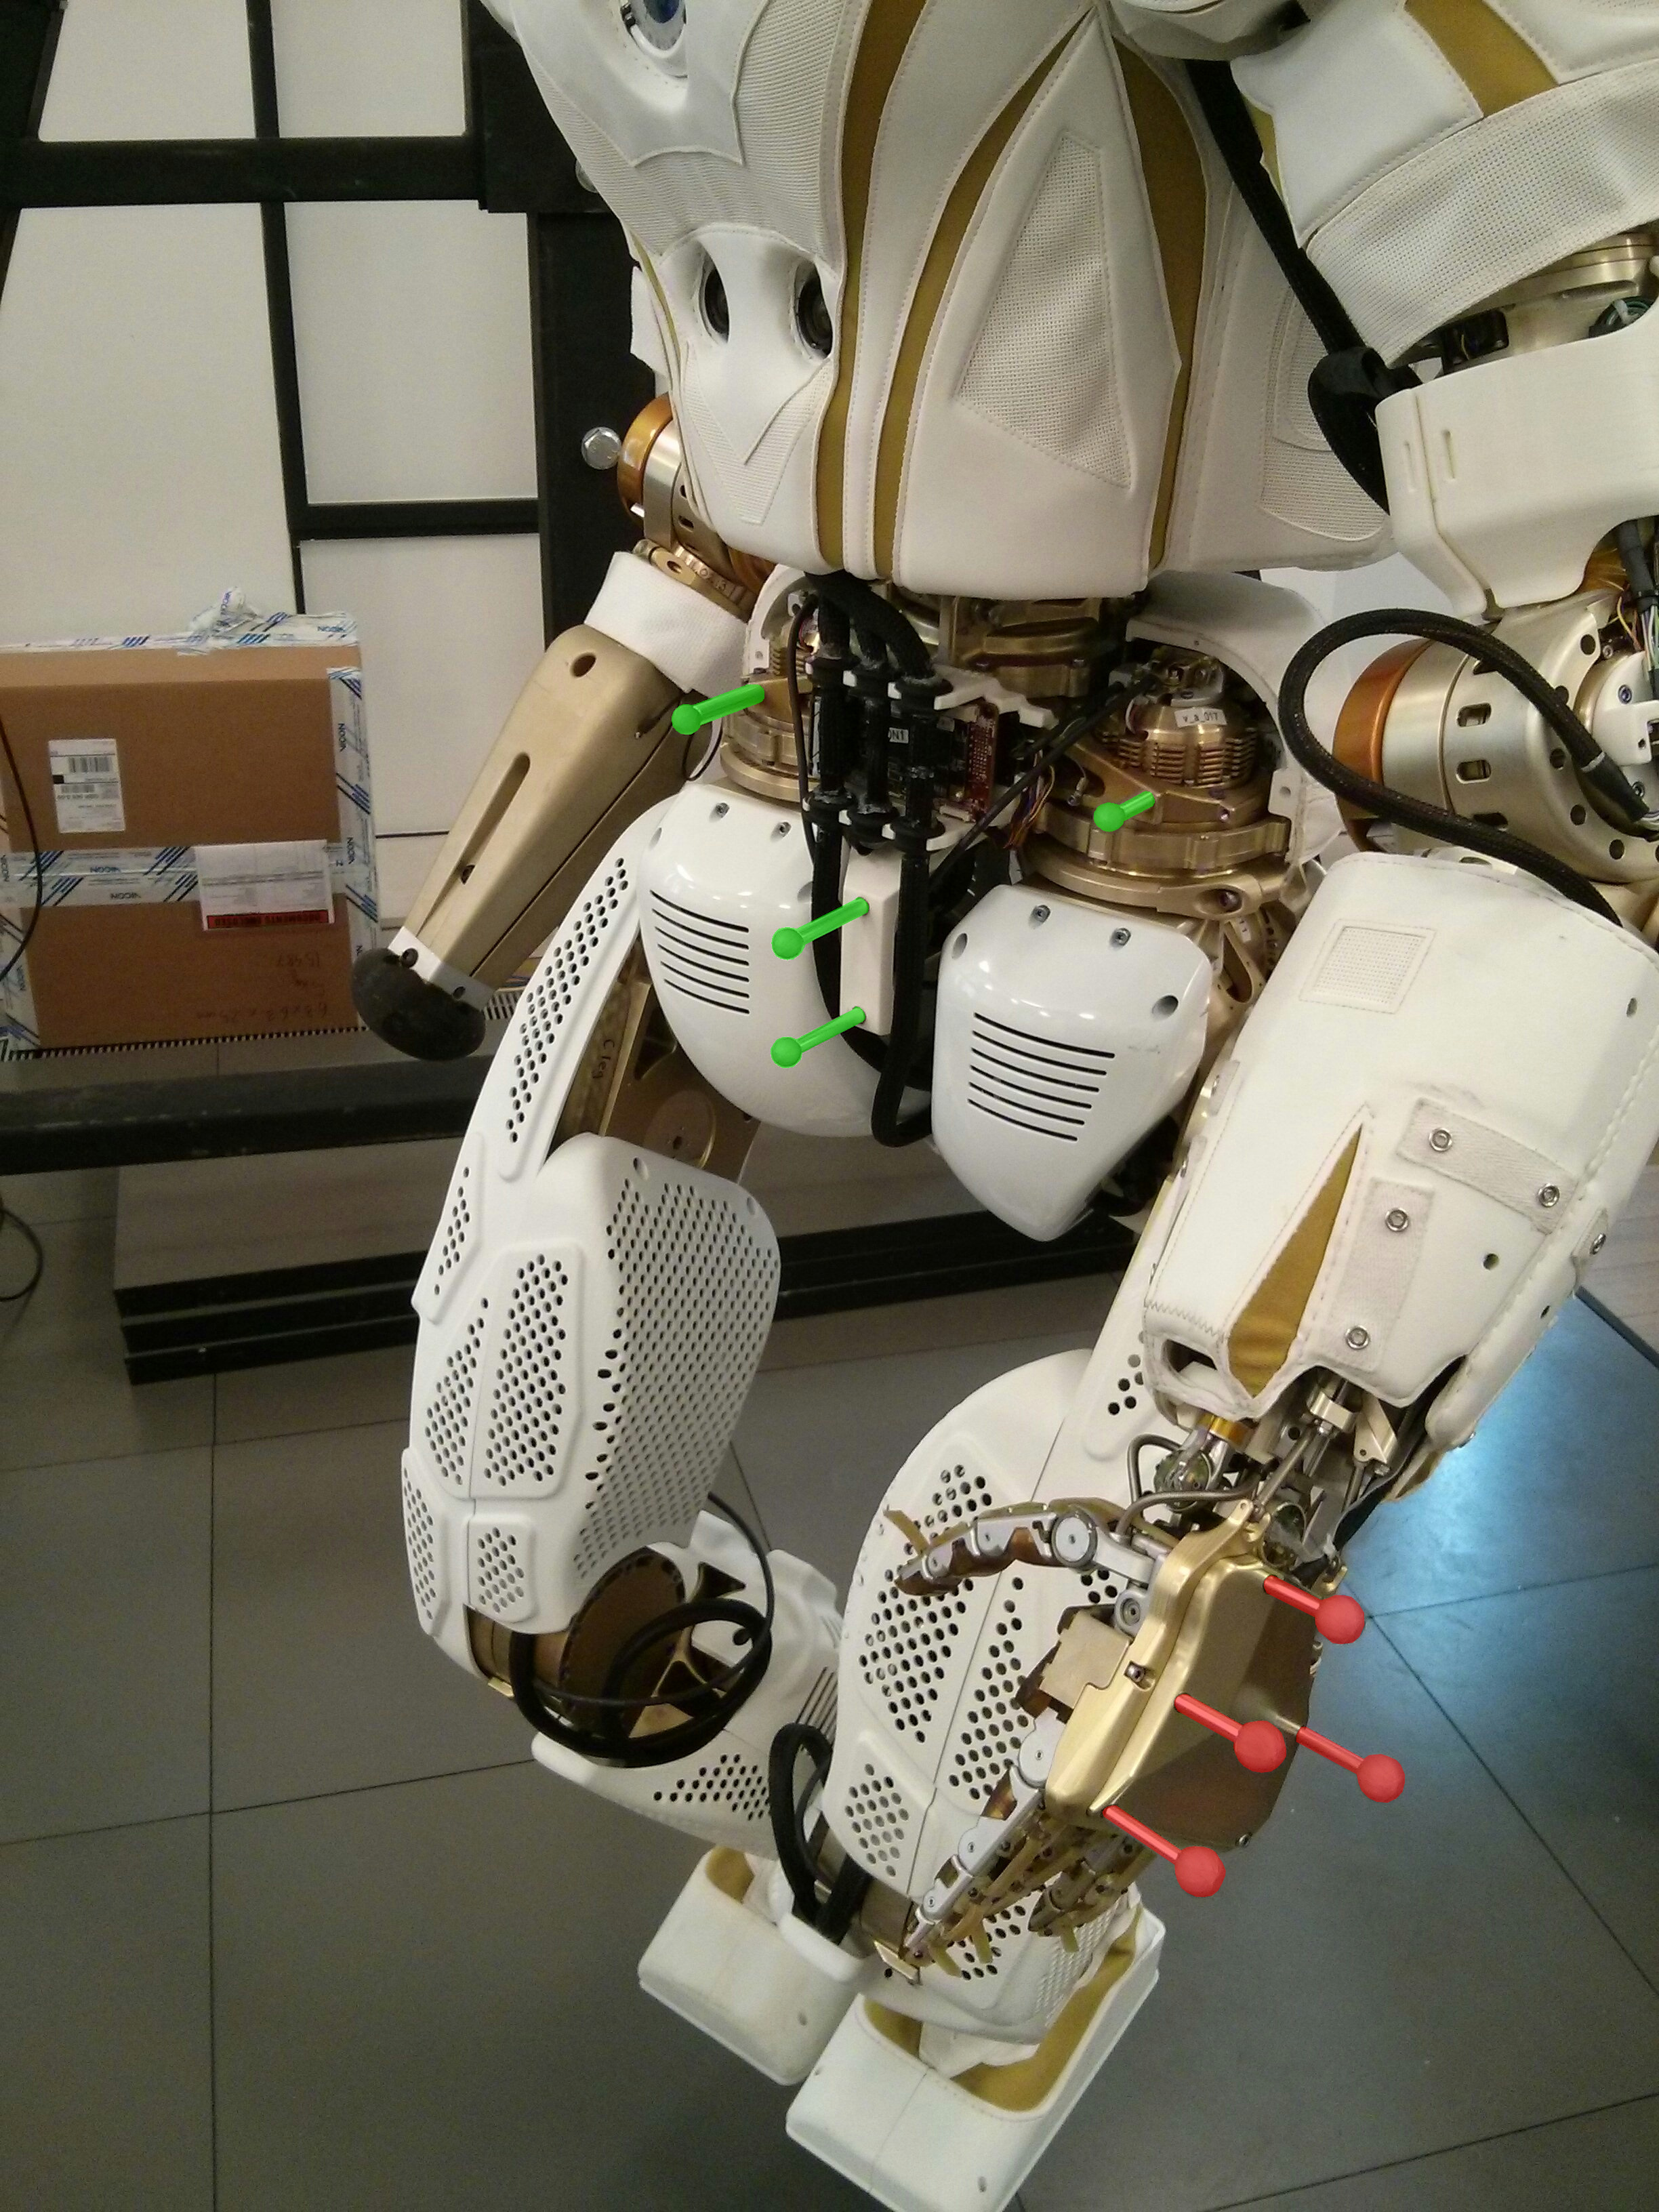
\includegraphics[width=0.4\textwidth]{images/vicon_pose/vicon_marker_col.jpg}
\caption[Location of Vicon marker]{Location of Vicon marker on pelvis (green) and left hand (red)}
\label{fig:vicon_marker}
\end{figure}


\subsection{Hand Pose}

Each group of markers has its own coordinate system with its origin in the centre.
The drawing in \cref{fig:transform_vicon_robot} visualizes the transformations between the Vicon world frame, the Vicon marker frames and the robot frames.
The transformations $T_{w \rightarrow vp}$ and $T_{w \rightarrow vh}$ are the reported poses of the Vicon marker in the world frame.
To obtain the transformation $T_{p \rightarrow h}$, which gives the hand pose in the pelvis frame, we need to find the rigid transformation between the Vicon marker and robot frame ($T_{m \rightarrow p}$ and $T_{m \rightarrow h}$).

\begin{figure}
\captionsetup{width=0.52\textwidth}
\centering
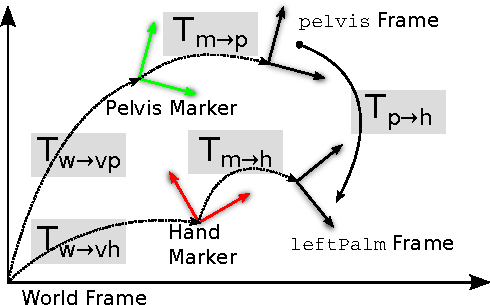
\includegraphics[width=0.5\textwidth]{images/vicon_pose/vicon_transforms.pdf}
\caption[Transformations of Vicon markers]{Transformations between Vicon markers (\textit{pelvis} - green, \textit{hand} - red) and robot frames}
\label{fig:transform_vicon_robot}
\end{figure}

The rigid transformation between marker and robot frames can be obtained by a least-squares optimization on corresponding points in both frames \cite{Umeyama1991}. Given corresponding points $m_i$ in marker frame and $x_i$ in the robot frame, the optimal projection of marker points from the marker frame into corresponding points in the robot frame becomes
\begin{equation}
T_{x \rightarrow m} = \arg\min_{R,t} \frac{1}{N} \sum_{i=1}^N \lVert x_i - \left( R \cdot m_i + t \right) \rVert_2
\label{eqn:least_squares_transformation_estimation}
\end{equation}
where $T_{x \rightarrow m}$ denotes the homogeneous transformation matrix containing the rotation matrix $R$ and the translation vector $t$. The points $x_i$ in the robot frame are here interchangeable for points $p_i$ in the \texttt{pelvis} frame and $h_i$ in the \texttt{leftPalm} frame.

%The Vicon system provides the pose of the marker frame in the world coordinate frame. That is the inverse of the transformations $T_{w \rightarrow vp}^{-1}$ and $T_{w \rightarrow vh}^{-1}$, e.g. the projection of the marker into the world frame.
The pose of the \texttt{pelvis} and \texttt{leftPalm} frame in the Vicon world frame can be expressed by the transformations
\begin{align}
T_{w \rightarrow p} &= T_{w \rightarrow vp} \cdot T_{p \rightarrow m} = T_{w \rightarrow vp} \cdot T_{m \rightarrow p}^{-1} \\
T_{w \rightarrow h} &= T_{w \rightarrow vh} \cdot T_{h \rightarrow m} = T_{w \rightarrow vh} \cdot T_{m \rightarrow h}^{-1} .
\end{align}

The transformations between these robot frames then finally becomes
\begin{align}
T_{w \rightarrow h} &= T_{w \rightarrow p} \cdot T_{p \rightarrow h} \\
T_{w \rightarrow vh} \cdot T_{m \rightarrow h}^{-1} &= T_{w \rightarrow vp} \cdot T_{m \rightarrow p}^{-1} \cdot T_{p \rightarrow h} \nonumber \\
T_{p \rightarrow h} &= \left( T_{w \rightarrow vp} \cdot T_{m \rightarrow p}^{-1} \right)^{-1} \cdot T_{w \rightarrow vh} \cdot T_{m \rightarrow h}^{-1} \label{eqn:hand_pose_from_vicon} .
\end{align}

Given the transformations of the Vicon markers ($T_{w \rightarrow vp}$ and $T_{w \rightarrow vh}$) at each time instance, and the rigid transformation between these markers and the robot frame ($T_{m \rightarrow p}$ and $T_{m \rightarrow h}$) we can recover the true pose of the hand in the pelvis frame ($T_{p \rightarrow h}$) using \cref{eqn:hand_pose_from_vicon}.


\subsection{Joint Position Offset Calibration}

The availability of a true transformation within the robot kinematic chain enables us to compare the reported hand pose from forward kinematics with the true hand hand pose and further, calibrate the joints in the kinematic chain such that this deviation is minimized.

For minimizing the joint position deviation and obtaining correction offsets, the same optimization approach as described in \cite{Fallon2015} is applied. That is, given a correction function that maps a reported joint position value to its corrected value: $f_{corr}: q_{rep,i} \mapsto q_{corr,i}$, and a mapping from this joint space configuration to the 	task space pose of the manipulator using forward kinematics $\phi: \mathbf{q} \mapsto \mathbf{p}$, with the pose $\mathbf{p} \in SE(3)$, the optimal correction parameters can be found by minimising
\begin{equation}
e = \frac{1}{N} \sum_{i=1}^N  \lVert \phi \left( f_{corr}(q_{rep,i}) \right) - \mathbf{p}_i \rVert_2
\end{equation}
for $N$ samples, respectively poses. The average error is selected over the summed error to have comparable costs between varying lengths of sample sequences.

Two correction function $f_{corr}$ have been selected. The constant correction
\begin{equation}
f_{corr}(q_{rep}) = q_{offset} + q_{rep}
\end{equation}
assumes constant offset that is independent from the reported joint position value itself. Here, only one parameter per calibrated joint is to be optimized. A linear correction function
\begin{equation}
f_{corr}(q_{rep}) = q_{offset} + m_1 \cdot q_{rep}
\end{equation}
assumes an additional relation to the reported joint position value itself. In this case twice the parameters are optimised.

To prevent overfitting of the optimized correction parameters on the data set, the optimization result must be applied to a dedicated test set that has not been used for optimization. This is especially the case for more complex correction functions.
